\documentclass{article}

% for images: png, pdf, etc
\usepackage{graphicx}

% for nice table formatting, i.e. /toprule, /midrule, etc
\usepackage{booktabs}

% for nice units
\usepackage{siunitx}

\usepackage{amsmath}

\title{Quiet Standing Controller Parameter Identification: A Comparison of
Methods}

\author{Jason K. Moore and Antonie van den Bogert}

\begin{document}

\maketitle

\section{Introduction}

It is hypothesized that a human operating during the quiet standing task uses
feedback to remain upright in the face of perturbations. For various reasons,
it is desirable to obtain mathematical models that predict a human's actuation
patterns given measured estimates of the sensory information available to the
human.  Reasonably good models of the human's open loop musculoskeletal system
exist but models of the human's control system and the system process noises
are still less than adequate. The control model can possibly be derived from
first principles, but high level understanding of the human's sensory
neurological feedback patterns are difficult to derive from the low level
neurological first principles. These high level control descriptions may be
more easily arrived at through identification and learning techniques.

Here we present a numerical study comparing three methods of identifying the
parameters of a human quiet standing state feedback system. The first method,
direct identification, is by far the least computationally intensive but
suffers from bias due to the unknown processes in the modeled
system~\cite{Kooij2010}. The second method, single shooting, is a typical
method for parameter identification but is the most computationally intensive
and often suffers from extreme sensitivity to initial guesses. Finally, the
third method, which has not been used for control parameter identification in
biological systems, is direct collocation. We aim to show that direct
collocation is better suited to control parameter identification because it
does not suffer from bias, computation times are very reasonable, and it is
much less sensitive to initial guesses than shooting.

\section{Musculoskeletal Model Description}

We make use of the widely used planar two link inverted pendulum model of human
quiet standing. In particular, our model matches that described in
\cite{Park2004}. Figure~\ref{fig:free-body-diagram} shows the open loop system.
The human is modeled by two rigid bodies: the legs and the torso. These are
connected to each other at the hip joint, modeled as an ideal pin. The legs can
rotate about a pin joint relative to the ``platform'' and the platform/ankle
point can be laterally accelerated. The centers of mass of the legs and torso
are located line connecting the respective pin joints. The muscles are modeled
as simple joint torque actuators. The orientation of the bodies are described
by the generalized coordinates $\theta_a$ and $\theta_h$. Gravity acts on the
bodies in the $-y$ direction. The equations of motion were formed symbolically
using Kane's Method \cite{Kane1985} using SymPy~\cite{Gede2013}. The model
derivation is included in the \verb|src/model.py| file and implemented in a
class named \verb|QuietStandingModel|.

The numerical values of the model constants were estimated using Yeadon's
method and the software package \verb|yeadon|~\cite{Dembia2014}. The
measurements are included in \verb|raw-data/yeadon-measurements.yml|.
Table~\ref{tab:model-constants} reports the computed constants for the model.

% TODO : This is too long!
\begin{equation}
  \begin{bmatrix}
  0 \\
  0 \\
  0 \\
  0
\end{bmatrix}
=
\begin{bmatrix}
\omega_{a} - \dot{\theta}_{a}\\
\omega_{h} - \dot{\theta}_{h}\\
d_{L} g m_{L} \operatorname{sin}\left(\theta_{a}\right) + d_{L} m_{L} a \operatorname{cos}\left(\theta_{a}\right) + d_{T} g m_{T} \operatorname{sin}\left(\theta_{a} + \theta_{h}\right) + d_{T} l_{L} m_{T} \left(\omega_{a} + \omega_{h}\right)^{2} \operatorname{sin}\left(\theta_{h}\right) - d_{T} l_{L} m_{T} \omega^{2}_{a} \operatorname{sin}\left(\theta_{h}\right) + d_{T} m_{T} a \operatorname{cos}\left(\theta_{a} + \theta_{h}\right) + g l_{L} m_{T} \operatorname{sin}\left(\theta_{a}\right) + l_{L} m_{T} a \operatorname{cos}\left(\theta_{a}\right) - \left(I_{T} + d_{T} m_{T} \left(d_{T} + l_{L} \operatorname{cos}\left(\theta_{h}\right)\right)\right) \dot{\omega}_{h} - \left(I_{L} + I_{T} + d_{L}^{2} m_{L} + m_{T} \left(d_{T}^{2} + 2 d_{T} l_{L} \operatorname{cos}\left(\theta_{h}\right) + l_{L}^{2}\right)\right) \dot{\omega}_{a} + T_{h}\\
d_{T} g m_{T} \operatorname{sin}\left(\theta_{a} + \theta_{h}\right) - d_{T} l_{L} m_{T} \omega^{2}_{a} \operatorname{sin}\left(\theta_{h}\right) + d_{T} m_{T} a \operatorname{cos}\left(\theta_{a} + \theta_{h}\right) - \left(I_{T} + d_{T}^{2} m_{T}\right) \dot{\omega}_{h} - \left(I_{T} + d_{T} m_{T} \left(d_{T} + l_{L} \operatorname{cos}\left(\theta_{h}\right)\right)\right) \dot{\omega}_{a} + T_{a}
\end{bmatrix}
\end{equation}

\begin{figure}
  \centering
  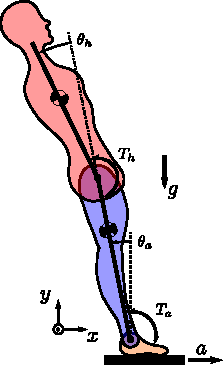
\includegraphics{figures/free-body-diagram.pdf}
  \caption{Free body diagram of musculoskeletal model used in this study.}
  \label{fig:free-body-diagram}
\end{figure}

\begin{table}
  \centering
  \caption{Constant parameters in the plant}
  
\begin{tabular}{llll}
  \toprule
  Variable & Description & Value & Units \\
  \midrule
$l_{L}$ & booger & 0.878 & \si{\meter} \\
$d_{L}$ & booger & 0.572 & \si{\meter} \\
$d_{T}$ & booger & 0.314 & \si{\meter} \\
$m_{L}$ & booger & 32.126 & \si{\kilogram} \\
$m_{T}$ & booger & 48.831 & \si{\kilogram} \\
$I_{L}$ & booger & 1.799 & \si{\kilogram\meter\squared} \\
$I_{T}$ & booger & 2.481 & \si{\kilogram\meter\squared} \\
$g$ & booger & 9.810 & \si{\meter\per\second\squared} \\
  \bottomrule
\end{tabular}
  \label{tab:model-constants}
\end{table}

\section{Control Model Description}

To close the loop, we assume the human's sensors allow for full state feedback.
There is physicoolgical backing for this assumption but we mostly choose it for
computational simplicity. Given the state vector:

\begin{equation}
  x = \left[\theta_a \theta_h \omega_a \omega_h \right]^T
\end{equation}

we can close the loop with

\begin{equation}
  T = K * (x_ref - x)
\end{equation}

Therefore we create a gain matrix:

\begin{equation}
  \begin{bmatrix}
    k_{00} & k_{01} & k_{02} & k_{03} \\
    k_{10} & k_{11} & k_{12} & k_{13} \\
  \end{bmatrix}
\end{equation}

The acceleration $a$ is treated as an exogenous input.

We consider a process noise, in our case we add noise to the reference. This
primarily represents the controller's error in estimatign the state error, but
can also

\section{Data Measurement}

Several variables are useful as measurements, $y_m$, for identification
purposes. To obtain the state trajectory under the two exongenous inputs $a$
and $x_n$, we simulate the system by integrating the first order form of the
equations of motion forward in time. We use the variable step integration
routine available in odepack's lsoda routine and acces it through SciPy's
integration wrappers. The measurements, $y$ are

\begin{equation}
  y_m(t) = [a(t), x(t), T(x)] + v(t)
\end{equation}

where v(t) is a random process vector with a mean of zero and standard
deviation.

\section{Direct Identification}

The direct approach can be used to identify the gains in the controller. The
accuracy of this approach relies heavily on the ratio of the system's process
noise and the applied pertrubations \cite{Kooij2005}. To implement the inputs
to the controller (-x) and the outputs of the controller (T) are assumed to be
measured. A linear identifcation model is constructed and linear least squares
can be used to compute the optimal gains for a set of measurments.

For the identification we assume that the controller model is:

\begin{equation}
  u = -K * x
\end{equation}

i.e. not affected by reference noise or deviating reference

Measuered states and joint torques
$\mathbf{X}$ : N x n
$\mathbf{T}$ : N x m

Unknown gains
$\tilde{\mathbf{K}}$: n x m

\begin{equation}
  -x \tilde{K} = \mathbf{T}
\end{equation}

The least squares estimation

\section{Indirect Identification: Shooting}

Indirect identification is based on minimizing the following cost function:

\begin{align}
  J(p) = \int_{t_0}^{t_f} [x_m(t) - x(t, p)]^2 dt
\end{align}

the state at any time is determined by integrating the eqations of motion

\begin{equation}
  x = \int_{t_0}^{t_f} f(x, t, r_m, p_m, p) dt
\end{equation}

$r_m$ : measured exongenous input
$p_m$ : measured constant parameters
p : unknown constant parameters

given the initial state $x_0$ \footnote{Here we assume that the initial state is
zero and do not include it in the objective's unknowns}.

To test shooting we make use both a gradient based sovler and a gradient free
evolutionary algorithm.

The quasi-Newton method of Broyden, Fletcher, Goldfarb, and Shanno is a common
general purpose minimizer for unconstrained problems. And we use the CMAES
algorithm which is has been successfully used for control identification
purposes \cite{Wang2010}.

\begin{equation}
  J(\tilde{K}) = h \sum_1^N (\bar{x}_i - x_i)^2
\end{equation}

\section{Indirect Identification: Direct Collocation}

We make use of direct collocation to transform the parameter identifaction
problem into a large scale non-linear programming problem. Do do so we first
assume that the discrete integral can be described by backward Euler
integration, giving an approximation of the state derivative as

\begin{align}
  x_{i} = x_{i-1} + h f(x_{i}, t_{i}) \\
  \dot{x} \approx \frac{x_i - x_{i-1}}{h} =  f(t_i, x_i)
\end{align}

For $t_i$ where $i=2 \dots N$ and the above assumption, we form $N-1$ algebraic
equations which must be satisfied.

\begin{align}
  0 = \mathbf{c}(\mathbf{\theta}) \\
  0 = f_i(x_{i}, x_{i-1}, u_i, p, h)
\end{align}

The objective function is the linear least squares norm which minimizes the
error in the measured data with respect to the model's trajectory.

\begin{equation}
  J(\theta) = h \sum_{i=1}^N \left[y_{mi} - y_i(\theta)\right]^2
\end{equation}

The NLP problem can be formed

\begin{align}
  \min_{\theta \in \Re^{n}}  J(\theta) \\
  c(\theta) = 0 \\
  \theta^L \leq \theta \leq \theta^U
\end{align}

The goal is to estimate the uknown parameters $p$, the controller gains in our
case, given noisy measurements, $y_{m_i}$.

\bibliographystyle{unsrt}
\bibliography{references}

\end{document}
